\section{Descrição do Algoritmo}

O algoritmo de George-Appel funciona através da construção de um grafo de interferência iterativo, e posteriormente, K-colorido, onde K é o número de registradores. Ao todo, possui sete etapas.\textit{ build, simplify, conservative coalesce, freeze, potential spill, select e actual spill}. Adota o estilo de Coalescência Conservadora de Briggs e a simplificação de Chaitin resultando em uma maior eficiência que ambas as técnicas separadas. A nova abordagem para alocação de registradores com grafos de interferência iterativo garante uma execução em loop das etapas, retomando, em laço, as etapas de simplficação, coalescência, congelamento e derramamento inúmeras vezes no mesmo grafo. Tal característica torna dificil estimar a complexidade do algoritmo.



\textit{Build:} Constrói o grafo de interferência e categoriza os vértices entre instruções de cópia (move related) ou não.


\textit{Simplify:}  Remove as instruções de cópia de menor grau no grafo.


\textit{Conservative Coalesce:} Atua semelhante ao algoritmo de Briggs.

\textit{Freeze: } Nem simplifica nem coalesce, busca instruções cópia de baixo grau e as congela. Retorna às etapas de simplificação e coalescência

\textit{Select: } Mesma etapa dos algoritmos anteriores, exceto que não adotada bias na hora do julgamento para otimização precoce de instrução de moves.

\textit{Spill: } Armazena as variáveis na memória RAM para retorná-las futuramente.

Uma instrução de cópia ( ou move instruction ) é quando uma variável está armazenada no registrador temporário de origem e passa ao registrador de destino ( onde será processada ).

\subsection{Pseudocódigo e Complexidade: }

Dado os retornos sucessivos à etapa de build, e as sucessivas iterações e interoperações entre etapas de congelamento, derramento, coalescência, simplificação e seleção. É de enorme dificuldade estimar a complexidade global do algoritmo.

O pseudocódigo utilizado fora o original do artigo de George-Appel et al, 1996, página 19 à 23.

\begin{center}
    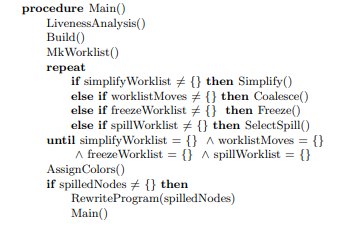
\includegraphics[scale=0.6]{img/code1.png}
    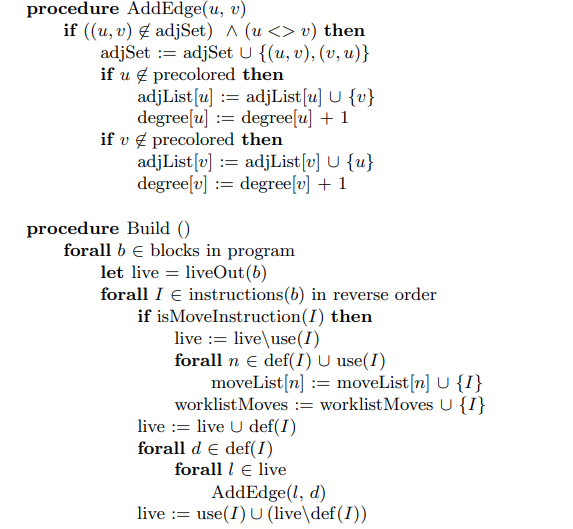
\includegraphics[scale=0.6]{img/code2.png}
    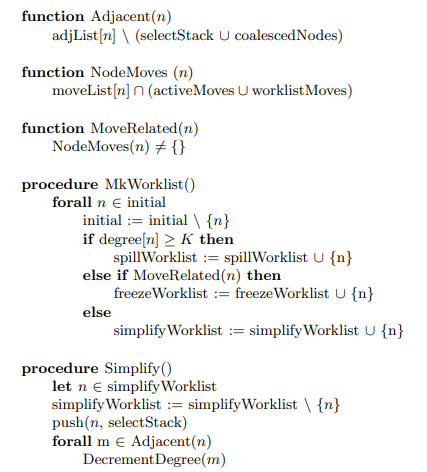
\includegraphics[scale=0.6]{img/code3.png}
    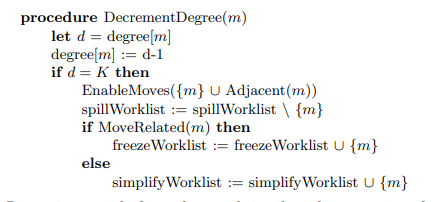
\includegraphics[scale=0.6]{img/code4.png}
    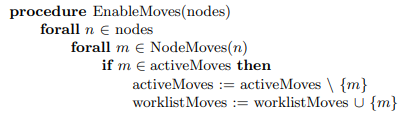
\includegraphics[scale=0.6]{img/code5.png}
    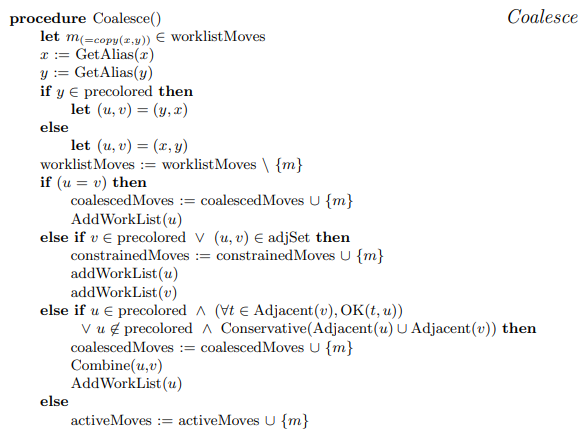
\includegraphics[scale=0.6]{img/code6.png}
    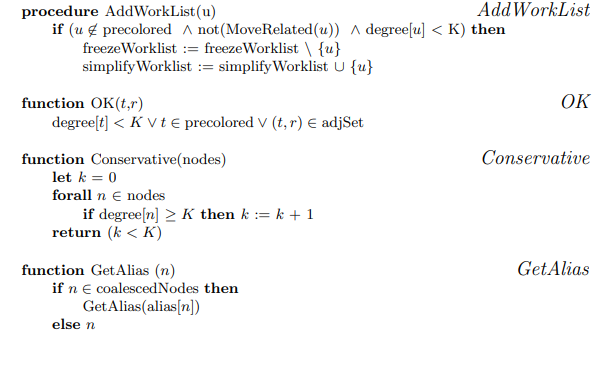
\includegraphics[scale=0.6]{img/code7.png}
    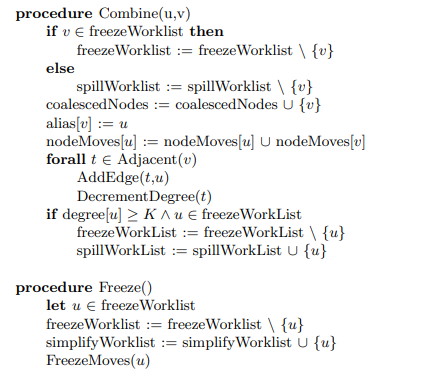
\includegraphics[scale=0.6]{img/code8.png}
    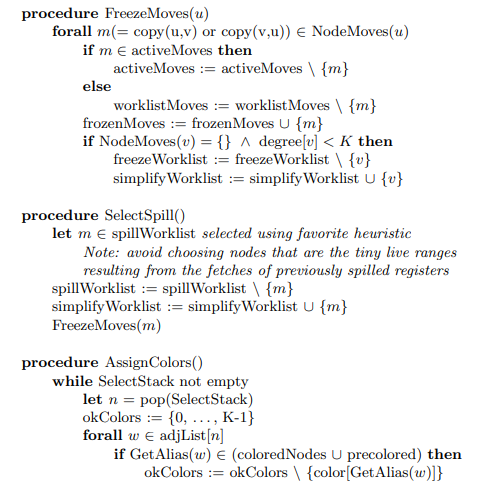
\includegraphics[scale=0.6]{img/code9.png}
    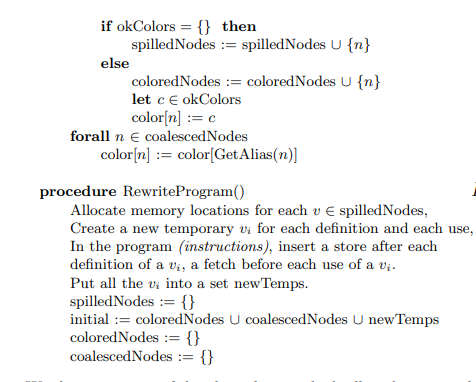
\includegraphics[scale=0.6]{img/code10.png}

\end{center}

Assume-se, que a instânciação do pseudocódigo ao algoritmo em uma linguagem de programação qualquer o implementador usará estruturas de dados eficientes para tal.

Seja A o número de arestas de interferência, V o número de vértices, K o número de registradores e M o número de instruções.

\textit{addEdge:} Abrevia-se a complexidade dessa instrução para $O(1)$.

\textit{Build:} Rotina responsável por criar os vértices e arestas, logo $O(V + A)$.

\textit{MkWorklist: } Itera até $n$ vezes o tamanho de $initial$, logo $O(n)$.

\textit{Simplify: } Dado um nó $n$, itera sobre seus vizinhos $adj(n)$, o que custa $O(d(n))$.

\textit{DecrementDegree: } Poucas comparações, justificamente análoga à addEdge.

\textit{EnableMoves: } Itera sobre os nós e a lista de instruções. Custo total $O(V + M)$.

\textit{Coalesce: } O custo de coalesce depende da complexidade dos vértices vizinhos chamados para a coalescência, logo $O(adj(u) + adj(v))$.

\textit{Combine: } Itera sobre todos os vertices pertencentes à adjacente, logo $O(d(vertice))$.

\textit{Freeze: } Custo $O(1)$ pois evoca FreezeMoves.

\textit{FreezeMoves: } Custo $O(M)$ pois itera o vetor do número de instruções.

\textit{SelectSpill: } Depende diretamente de quanto derramamento será causado no programa, pode ser $O(1)$ ou $O(V)$.

\textit{AssignColors: } Irá atribuir cores a todos vértices, logo $O(V)$.


A soma das complexidades individuais não representa a complexidade global do algoritmo, dado que o processo iterativo ocorre inúmeras vezes e chamadas de congelamento, derramamento, simplificação ocorrem inúmeras vezes no mesmo código.
